\chapter{System Design and Research Methodology}

\section{Introduction and Design Overview}

This chapter presents the system design and research methodology for empirical comparison of GitOps and Traditional CI/CD methodologies through the TechMart multi-cloud e-commerce platform. The design addresses dual requirements of providing a functional e-commerce platform while serving as a controlled research environment for rigorous methodology evaluation.

The system design prioritizes authenticity, scalability, and observability to enable comprehensive data collection while demonstrating enterprise-grade DevOps practices. The architecture deliberately distributes services across different platforms to create realistic operational complexity while enabling direct methodology comparison under identical business requirements.

The research methodology framework provides systematic approaches for data collection, complexity normalization, and statistical analysis that enable valid conclusions about methodology performance characteristics while accounting for service complexity variations and operational factors.

\section{Microservices Architecture Design}

\subsection{Service Architecture Overview}

The TechMart platform implements a four-service microservices architecture with strategic technology diversity reflecting real-world enterprise environments. The service decomposition follows domain-driven design principles with clear business capability boundaries and deliberate technology stack variation enabling comprehensive methodology evaluation.

\textbf{Service Architecture Comparison:}

\begin{table}[H]
\centering
\caption{Service Architecture and Technology Distribution}
\label{tab:service-architecture-comparison}
\begin{tabular}{|p{2.5cm}|p{3cm}|p{1.5cm}|p{2.5cm}|p{4cm}|}
\hline
\textbf{Service} & \textbf{Technology Stack} & \textbf{Complexity Score} & \textbf{Deployment Method} & \textbf{Key Capabilities} \\
\hline
User Service & Python FastAPI + PostgreSQL & 7.8/10 & GitOps (GKE) & Authentication, JWT, RBAC \\
\hline
Order Service & Python FastAPI + PostgreSQL + Redis & 8.2/10 & GitOps (GKE) & Transaction processing, Multi-DB \\
\hline
Product Service & Node.js Express + MongoDB & 5.4/10 & Traditional (Heroku) & Catalog management, Search \\
\hline
Cart Service & Java Spring Boot + Redis & 7.5/10 & Traditional (Heroku) & Reactive streams, Session mgmt \\
\hline
\end{tabular}
\end{table}

\begin{figure}[H]
\centering
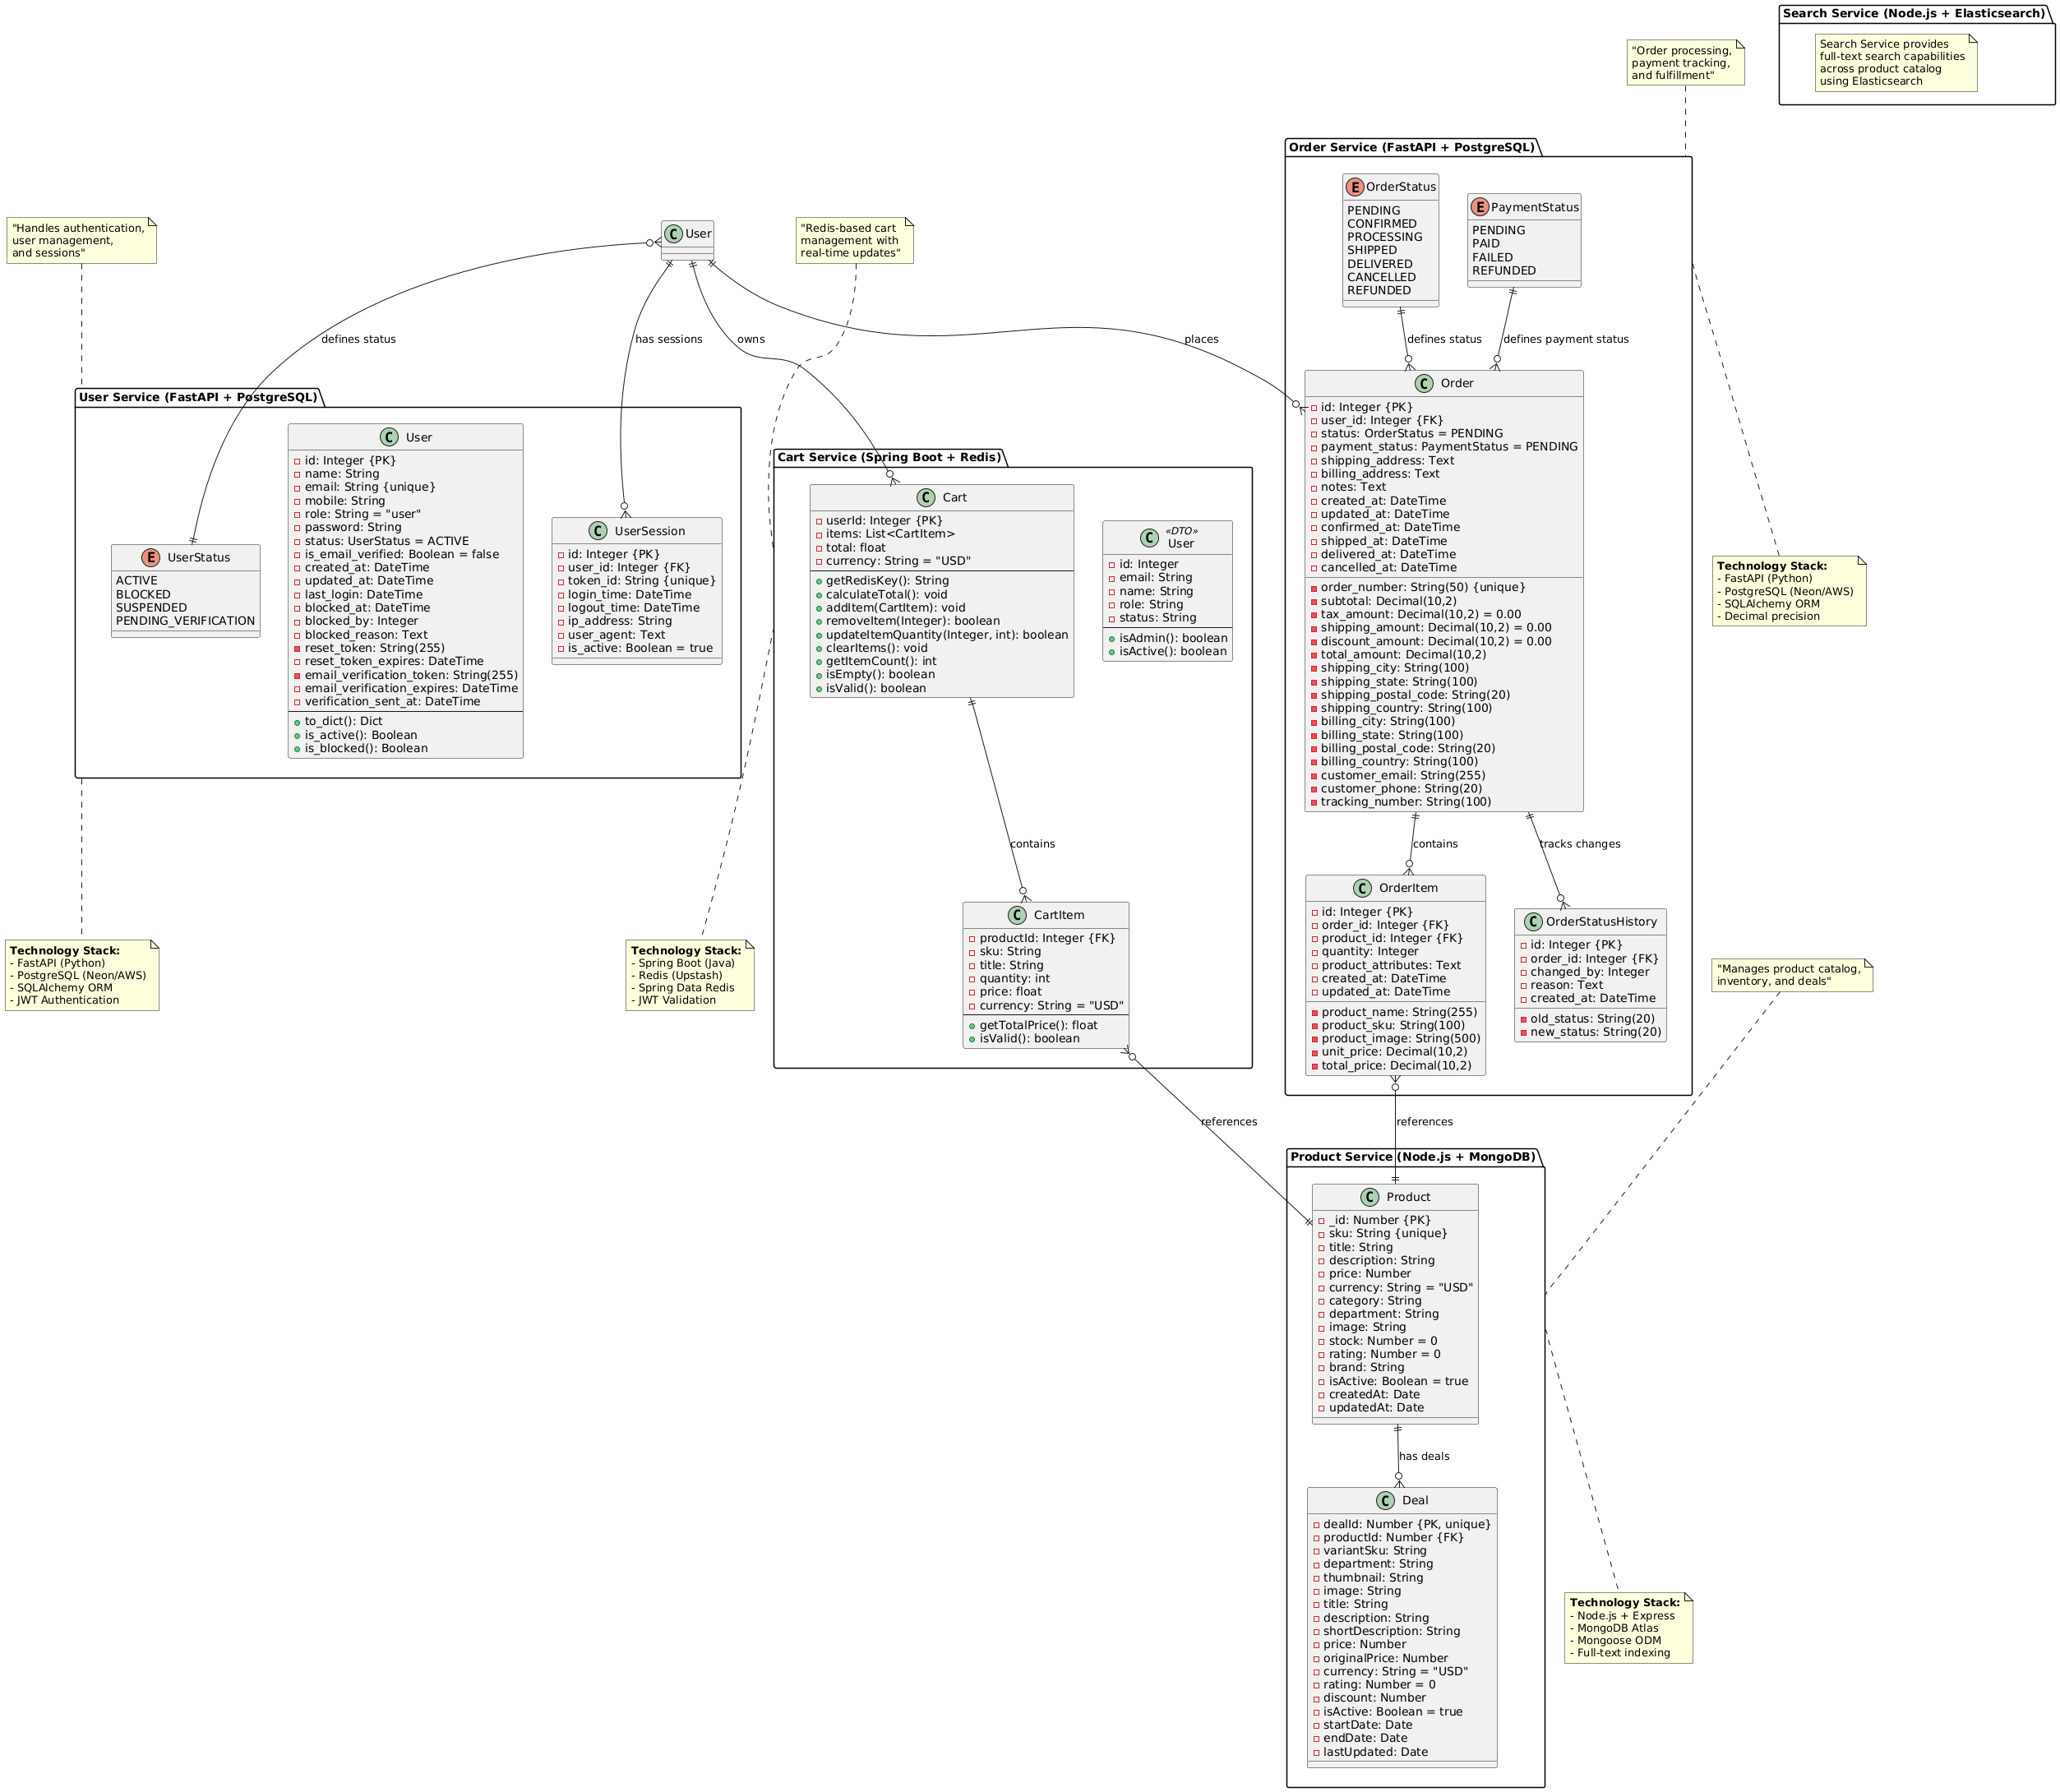
\includegraphics[width=0.9\textwidth]{figures/chapter4/class-diagram.png}
\caption{TechMart Platform Class Diagram showing database relationships and entity structure}
\label{fig:class-diagram}
\end{figure}

\textbf{Technology Selection Rationale:}
\begin{itemize}
\item \textbf{Python FastAPI:} Modern async framework for complex business logic (User/Order services)
\item \textbf{Node.js Express:} Lightweight platform optimization for Traditional CI/CD (Product service)
\item \textbf{Java Spring Boot:} Enterprise reactive patterns for high-performance operations (Cart service)
\item \textbf{Database diversity:} PostgreSQL (ACID), MongoDB (flexibility), Redis (performance)
\end{itemize}

\textbf{Service Complexity Framework:}
The complexity scoring accounts for codebase complexity (20\%), build requirements (25\%), resource intensity (20\%), technology stack characteristics (15\%), external dependencies (10\%), and deployment target complexity (10\%). This enables fair methodology comparison across heterogeneous service architectures.

\begin{figure}[h]
\centering
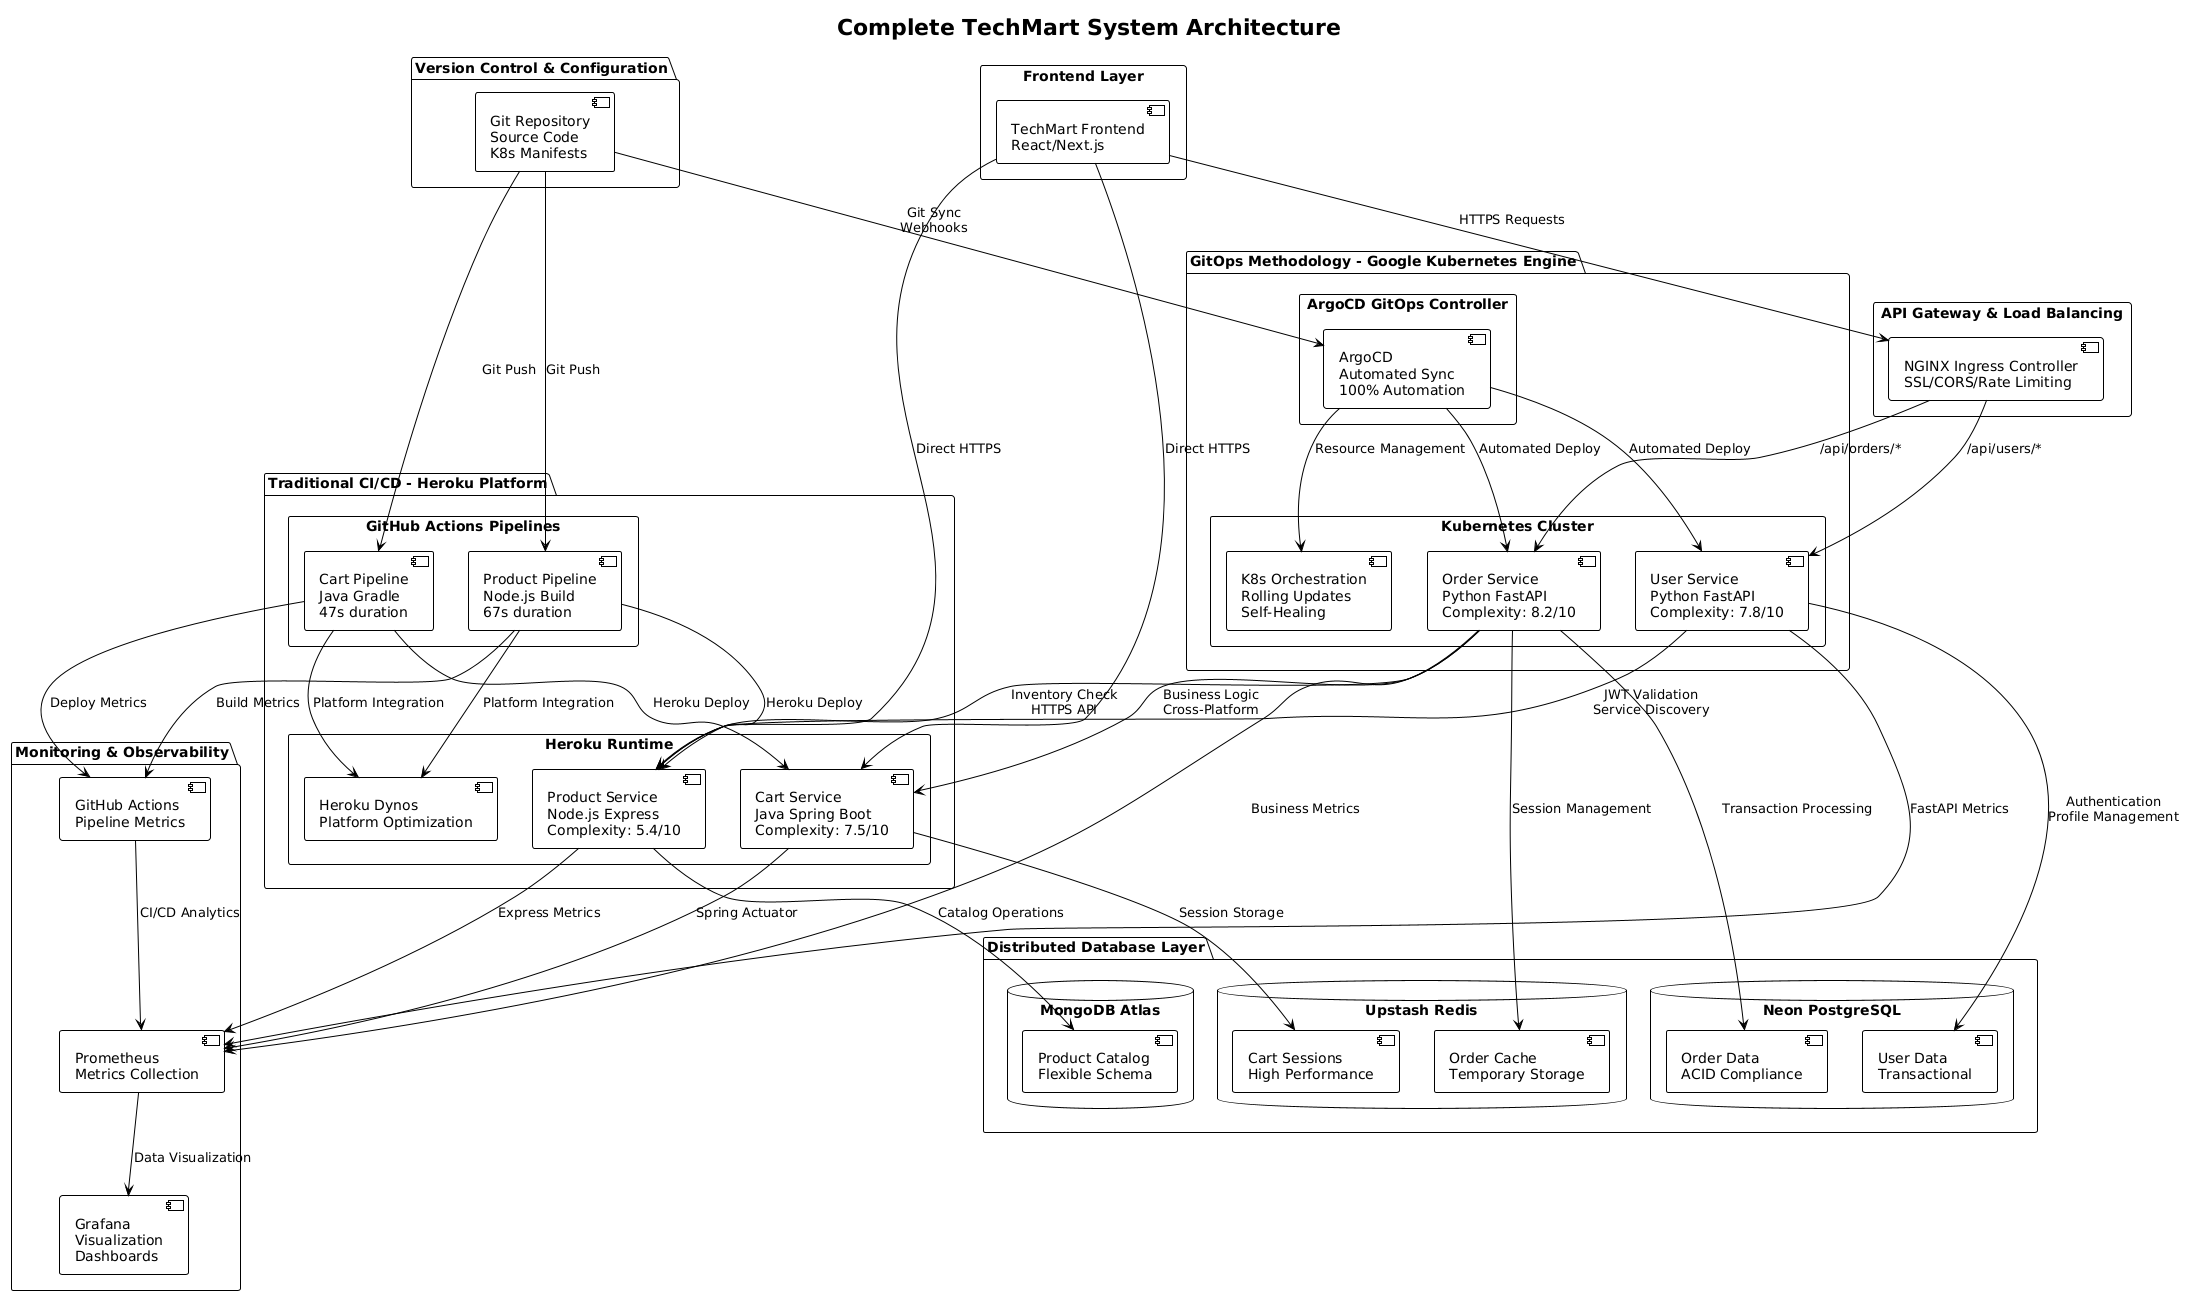
\includegraphics[width=1.0\textwidth]{figures/Complete-System-Architecture-Diagram.png}
\caption{Complete TechMart System Architecture}
\label{fig:complete-system-architecture}
\end{figure}

\begin{figure}[H]
\centering
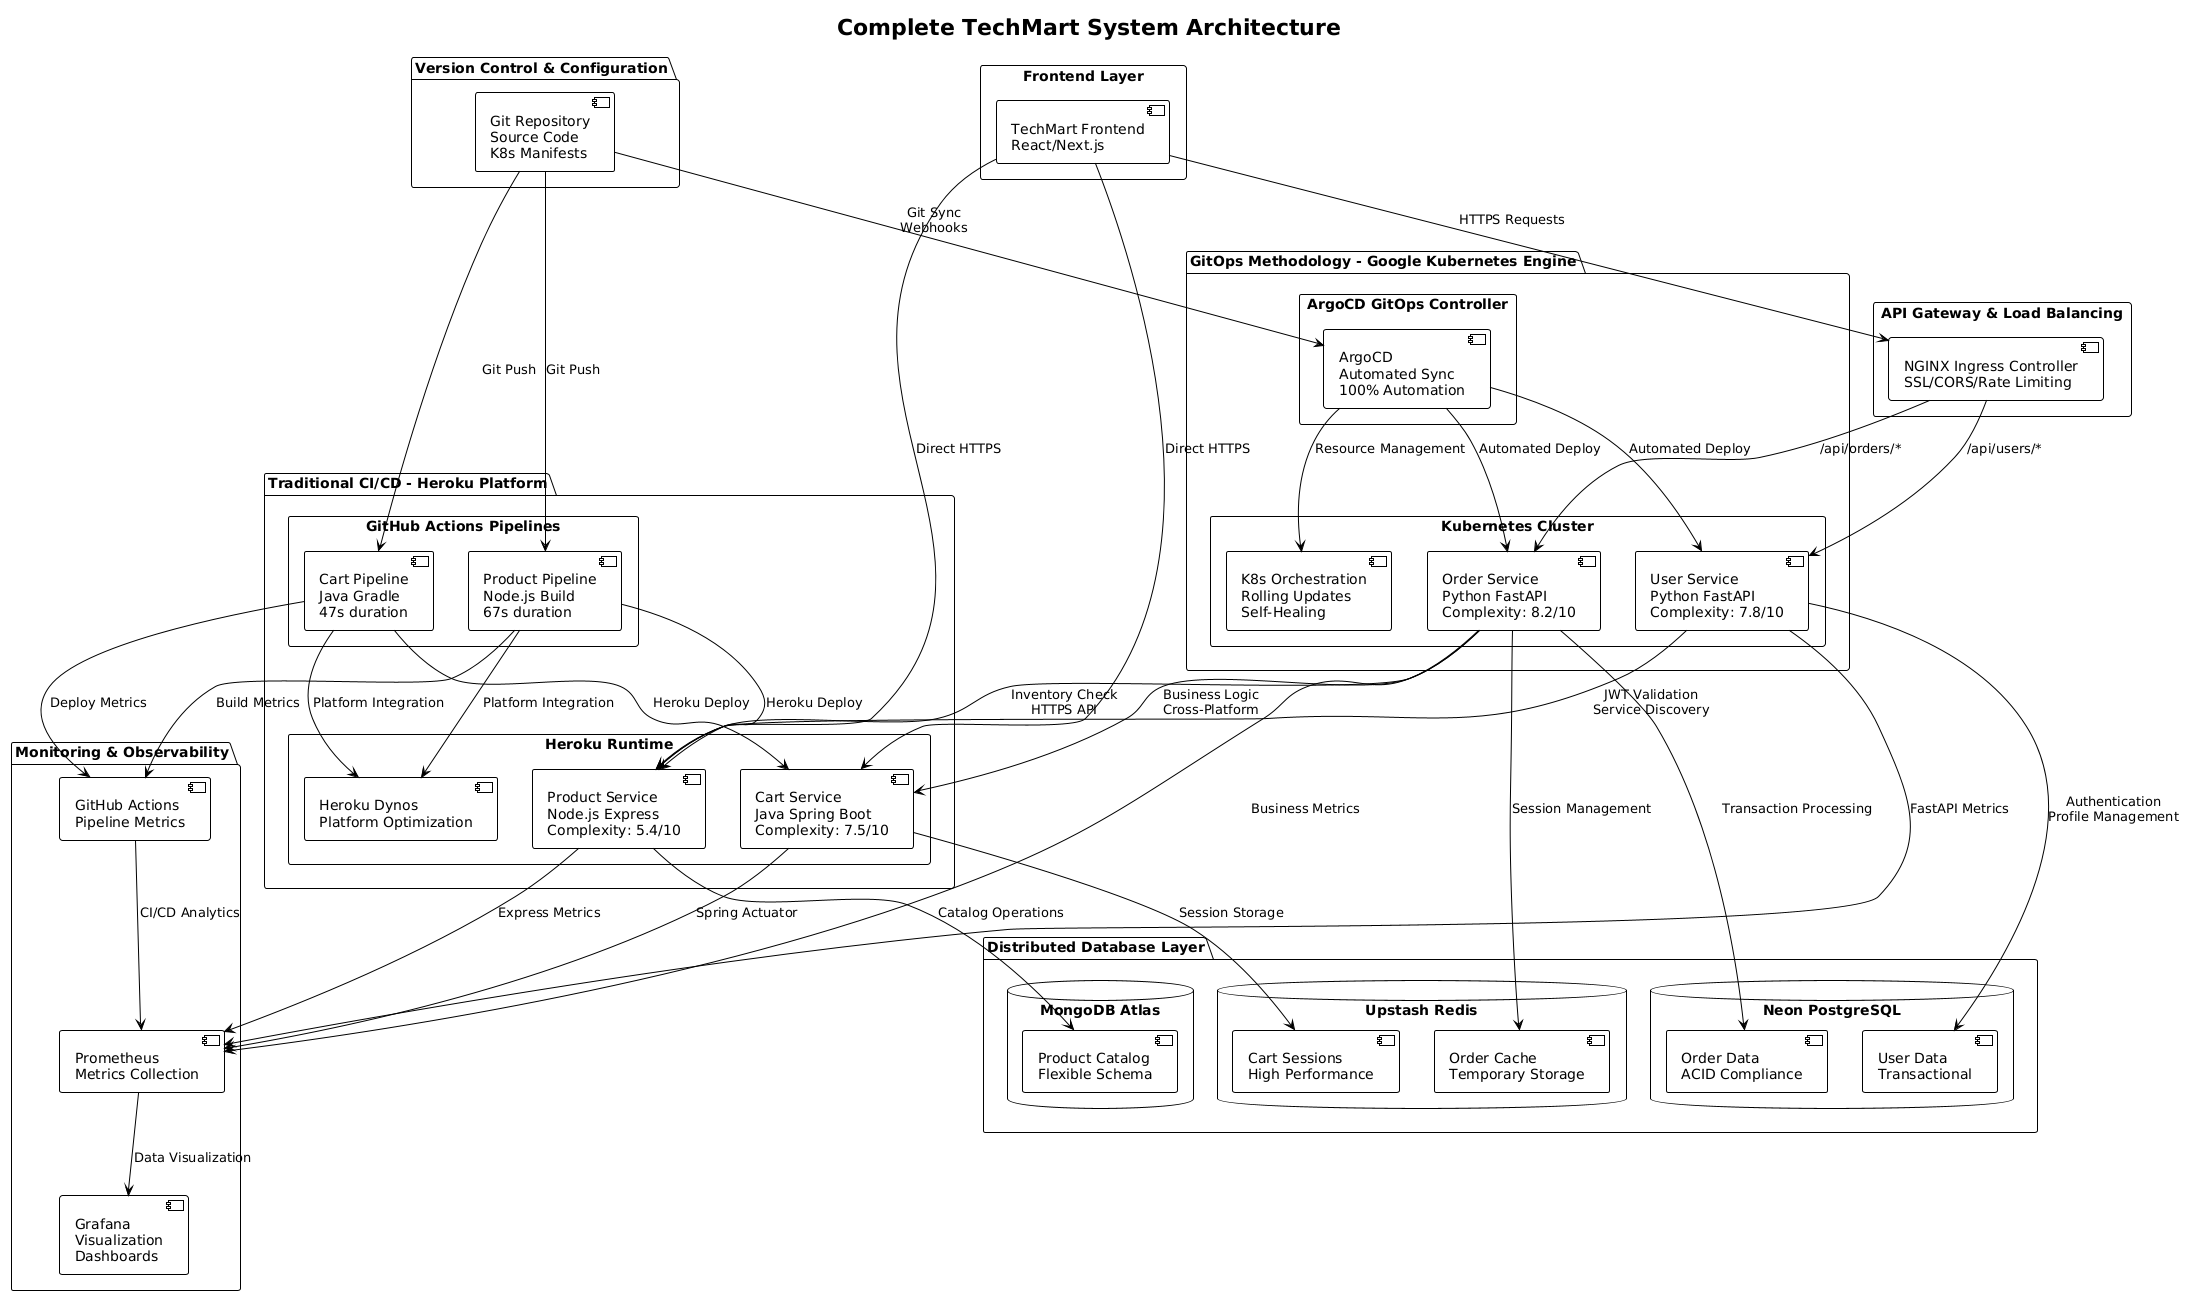
\includegraphics[width=1.0\textwidth]{figures/Complete-System-Architecture-Diagram.png}
\caption{Complete TechMart System Architecture}
\label{fig:complete-system-architecture}
\end{figure}

\subsection{Inter-Service Communication Architecture}

The microservices architecture implements sophisticated communication patterns demonstrating enterprise-grade integration while maintaining service autonomy. The communication design balances performance, reliability, and security requirements while enabling comprehensive observability for research data collection.

\subsubsection{Authentication Flow and JWT Integration}

The authentication architecture implements centralized JWT-based security where the User Service serves as the primary authentication provider for all platform services. This design demonstrates secure multi-service authentication while maintaining stateless communication patterns.

\textbf{Authentication Sequence:}
\begin{enumerate}
\item User Service generates JWT token with user claims and role assignments
\item Client includes JWT in Authorization headers for all service requests
\item Each service validates JWT signature using shared secret (HS256 algorithm)
\item Services enforce role-based access control based on JWT claims
\item Cross-service calls propagate authentication context for chained operations
\end{enumerate}

\textbf{JWT Token Structure:}
\begin{verbatim}
{
  "sub": "user_id_123",
  "email": "user@example.com",
  "name": "John Doe", 
  "role": "user|admin",
  "iat": 1692123456,
  "exp": 1692125256,
  "jti": "unique_token_id"
}
\end{verbatim}

\textbf{Security Implementation:}
\begin{itemize}
\item JWT tokens with 30-minute expiration and automatic refresh mechanisms
\item Shared secret key across all services for consistent token validation
\item Role-based access control with User and Admin privilege levels
\item CORS configuration enabling secure cross-origin requests from frontend
\item Comprehensive audit trail generation through request/response logging
\end{itemize}

\subsubsection{Business Transaction Patterns}

The platform implements complex business transactions spanning multiple services, demonstrating distributed transaction management and eventual consistency patterns essential for microservices architectures.

\textbf{Order Processing Transaction Flow:}
\begin{enumerate}
\item Cart Validation: Cart Service validates items and calculates totals
\item User Authentication: User Service validates customer identity and permissions
\item Product Verification: Product Service confirms availability and pricing
\item Order Creation: Order Service creates transaction records and manages state
\item Inventory Update: Product Service updates stock levels and availability
\item Payment Processing: Order Service coordinates with external payment providers
\item Fulfillment Initiation: Order Service triggers shipping and tracking processes
\end{enumerate}

\textbf{Data Consistency Management:}
\begin{itemize}
\item Event-driven architecture with service-to-service communication
\item Compensating transaction patterns for rollback scenarios
\item Eventual consistency models with conflict resolution strategies
\item Distributed state management with service ownership boundaries
\item Comprehensive error handling and retry mechanisms for transaction resilience
\end{itemize}

\section{Multi-Cloud Deployment Architecture}

The TechMart platform implements sophisticated multi-cloud deployment architecture demonstrating practical implementation of both GitOps and Traditional CI/CD methodologies across diverse cloud platforms. This heterogeneous deployment approach provides the controlled experimental environment necessary for rigorous methodology comparison.

The deployment architecture spans multiple cloud providers, each selected for specific technical characteristics and deployment patterns reflecting real-world enterprise requirements. The architectural design deliberately separates GitOps-deployed services (User and Order services on GKE) from Traditional CI/CD-deployed services (Product and Cart services on Heroku) to create controlled methodology comparison conditions.

\subsection{GitOps Architecture Design (GKE + ArgoCD)}

The GitOps implementation represents the platform's most sophisticated deployment pattern, utilizing Google Kubernetes Engine (GKE) with ArgoCD for declarative infrastructure management and continuous deployment. This architecture demonstrates advanced cloud-native practices with complete automation, self-healing capabilities, and declarative configuration management.

\subsubsection{ArgoCD Application Management}

The GitOps deployment utilizes two dedicated ArgoCD applications configured for maximum automation and reliability. Both User Service application (user-service-app-clean) and Order Service application (order-service-app) implement identical GitOps patterns with 100\% automation levels and comprehensive self-healing capabilities.

\textbf{ArgoCD Configuration Features:}
\begin{itemize}
\item Automated sync policies eliminating manual intervention requirements
\item Automatic pruning of obsolete resources with comprehensive cleanup
\item Self-healing capabilities automatically correcting configuration drift
\item Comprehensive rollback mechanisms with 10-revision history limits
\item Continuous synchronization with multicloud-gitops-research branch
\item Research labels enabling methodology performance tracking
\end{itemize}

The ArgoCD configuration includes specialized research labels with automation level indicators set to "100" and rollback capability flags for comprehensive deployment analysis. These labels facilitate automated collection of GitOps-specific performance metrics essential for methodology comparison research.



\subsubsection{Kubernetes Infrastructure Configuration}

The GitOps services deploy on sophisticated Kubernetes infrastructure optimized for production reliability and research data collection. Both services implement rolling update strategies with zero-downtime deployment patterns, maintaining service availability during updates through maxUnavailable: 0 and maxSurge: 1 configurations.

\textbf{Resource Allocation Strategy:}

\begin{table}[H]
\centering
\caption{Kubernetes Resource Allocation and Configuration}
\label{tab:kubernetes-resource-allocation}
\begin{tabular}{|p{3cm}|p{2.5cm}|p{2.5cm}|p{3cm}|p{3cm}|}
\hline
\textbf{Service} & \textbf{Memory Request/Limit} & \textbf{CPU Request/Limit} & \textbf{Health Probes} & \textbf{Special Configuration} \\
\hline
User Service & 128Mi/256Mi & 100m/200m & Liveness, Readiness, Startup & Kubernetes Secrets for DB \\
\hline
Order Service & 256Mi/512Mi & 150m/300m & Extended startup probes & Multi-service connectivity \\
\hline
\end{tabular}
\end{table}

Both services implement comprehensive health checking with extended startup probe configurations reflecting service initialization complexity. The startup probes include 30-40 failure thresholds with 10-15 second intervals, ensuring reliable service availability detection during GitOps deployment cycles.

\subsubsection{API Gateway and Ingress Management}

The GitOps architecture implements sophisticated NGINX Ingress Controller providing centralized API gateway functionality for the entire multi-cloud platform. The ingress configuration demonstrates advanced routing patterns with comprehensive CORS management enabling secure cross-origin communication.

\textbf{Advanced Ingress Features:}
\begin{itemize}
\item SSL termination through Let's Encrypt certificates with automatic renewal
\item Sophisticated routing rules supporting both User and Order Service endpoints
\item Comprehensive CORS configuration for multi-platform integration
\item Connection limiting (20 concurrent connections) and rate limiting (100 RPS)
\item Optimized timeout settings (60-second timeouts) and request size limits (10MB)
\item Upstream hashing for consistent load distribution
\end{itemize}

\subsection{Traditional CI/CD Architecture Design (Heroku)}

The Traditional CI/CD implementation demonstrates conventional deployment patterns utilizing Heroku Platform-as-a-Service for container orchestration and deployment automation. This architecture provides the controlled comparison baseline for evaluating GitOps methodology advantages while showcasing mature CI/CD practices.

\subsubsection{GitHub Actions Workflow Implementation}

The Traditional CI/CD implementation utilizes sophisticated GitHub Actions workflows demonstrating comprehensive automation while maintaining operational control points essential for enterprise deployment governance. The workflows implement multi-stage pipeline patterns with precise timing measurement for research analysis.

\textbf{Traditional CI/CD Pipeline Stages:}

\begin{table}[H]
\centering
\caption{Traditional CI/CD Pipeline Stage Comparison}
\label{tab:traditional-pipeline-stages}
\begin{tabular}{|p{3cm}|p{3cm}|p{3cm}|p{5cm}|}
\hline
\textbf{Service} & \textbf{Build Technology} & \textbf{Average Duration} & \textbf{Key Characteristics} \\
\hline
Product Service & Node.js + npm & 67 seconds & NPM dependency management, optional testing, Docker Hub integration \\
\hline
Cart Service & Java + Gradle & 47 seconds & Gradle caching, Spring Boot packaging, JVM optimization \\
\hline
\end{tabular}
\end{table}

\textbf{Product Service Traditional Pipeline (Task 1C):}
The Product Service implements Node.js-specific automation with comprehensive NPM dependency management, optional testing with graceful project accommodation, and Docker Hub image building with comprehensive tagging strategies. The pipeline demonstrates platform-native optimization with Heroku Container Registry integration.

\textbf{Cart Service Traditional Pipeline (Task 1D):}
The Cart Service implements Java Spring Boot automation with sophisticated Gradle build management, comprehensive dependency caching, and JAR compilation with Spring Boot optimization. The pipeline includes extensive testing capabilities and specialized Java application configuration.

\subsubsection{Heroku Platform Integration}

The Traditional CI/CD services deploy on Heroku Platform-as-a-Service, demonstrating mature cloud platform integration patterns with comprehensive operational capabilities. Heroku provides managed runtime environments with automatic scaling, integrated monitoring, and comprehensive operational tooling.

\textbf{Platform Integration Benefits:}
\begin{itemize}
\item Heroku Node.js buildpack with comprehensive dependency management
\item Java Spring Boot optimization with JVM tuning and memory management
\item Integrated MongoDB Atlas and Redis connectivity
\item Automatic SSL certificate management and domain routing
\item Comprehensive production logging and monitoring integration
\item Automated backup management and security patching
\end{itemize}

\subsection{Hybrid Integration Patterns}

The TechMart platform implements sophisticated hybrid integration patterns enabling seamless communication and data flow between GitOps-deployed services on Kubernetes and Traditional CI/CD-deployed services on Heroku. These integration patterns demonstrate enterprise-grade multi-cloud connectivity while maintaining security and performance characteristics.

\subsubsection{Cross-Platform Service Discovery and Communication}

The hybrid integration implements sophisticated service discovery patterns enabling reliable communication between services deployed across different cloud platforms and deployment methodologies. The service discovery architecture accommodates the dynamic nature of Kubernetes deployments while maintaining reliable connectivity to static Heroku endpoints.

\textbf{Service Discovery Implementation:}
\begin{itemize}
\item GitOps services utilize Kubernetes-native service discovery for internal communication
\item External service discovery patterns for Heroku-deployed services
\item Order Service maintains direct HTTPS connectivity to Cart and Product services
\item API Gateway provides centralized service discovery coordination
\item Comprehensive DNS-based resolution with health checking and failover
\end{itemize}

\subsubsection{Authentication and Authorization Propagation}

The hybrid architecture implements sophisticated authentication propagation patterns maintaining consistent security policies across GitOps and Traditional CI/CD deployed services. JWT token propagation implements shared secret validation across all platform services, enabling stateless authentication that scales across multi-cloud deployments.

\textbf{Cross-Platform Security Integration:}
\begin{itemize}
\item User Service on GKE serves as primary authentication provider
\item JWT tokens maintain validity across Heroku-deployed services
\item Consistent role-based access control policies across deployment methodologies
\item Comprehensive CORS management for secure cross-origin communication
\item Unified security boundaries regardless of deployment platform
\end{itemize}

\section{Infrastructure as Code and DevOps Patterns}

The TechMart platform implements comprehensive Infrastructure as Code (IaC) practices enabling reproducible, version-controlled, and automated infrastructure management across multiple cloud platforms. The IaC implementation demonstrates enterprise-grade DevOps practices while supporting both GitOps and Traditional CI/CD methodologies.

\subsection{Container Architecture and Multi-Stage Builds}

The platform implements sophisticated Docker containerization strategies optimizing for security, performance, and maintainability while accommodating diverse technology stacks. The container architecture demonstrates best practices for multi-stage builds, security hardening, and runtime optimization.

\subsubsection{Technology-Specific Container Optimization}

\textbf{Python FastAPI Containers (User/Order Services):}
\begin{itemize}
\item Alpine Linux base images for minimal attack surface and reduced size
\item Pipenv dependency management for reproducible Python environments
\item Comprehensive system dependency installation for cryptography and SSL
\item Application-level health checking endpoints for container orchestration
\item Proper signal handling and graceful shutdown for Kubernetes deployment
\end{itemize}

\textbf{Node.js Express Containers (Product/Search Services):}
\begin{itemize}
\item Node.js 18 Alpine base images providing optimal functionality-security balance
\item Efficient dependency installation with package.json-based management
\item NPM caching optimization for improved build performance
\item Lightweight containerization suitable for microservices deployment
\end{itemize}

\textbf{Java Spring Boot Container (Cart Service):}
\begin{itemize}
\item Multi-stage build processes optimizing image size while maintaining functionality
\item Gradle-based build automation with dependency caching and JAR compilation
\item Security-hardened Java 17 Alpine with non-root user execution
\item Spring Boot Actuator health checking and optimized JVM configuration
\item Advanced containerization with resource constraint awareness
\end{itemize}

\subsection{Kubernetes Manifests and Declarative Configuration}

The GitOps implementation utilizes comprehensive Kubernetes resource definitions demonstrating enterprise-grade container orchestration with advanced deployment strategies, resource management, and service discovery capabilities.

\subsubsection{Deployment Resource Configuration}

The GitOps services implement sophisticated Kubernetes Deployment resources demonstrating advanced container orchestration with comprehensive reliability and security features. Both services implement rolling update strategies with zero-downtime deployment capabilities.

\textbf{Deployment Configuration Features:}
\begin{itemize}
\item Rolling update strategies with maxUnavailable: 0 and maxSurge: 1
\item Comprehensive resource allocation with properly configured requests and limits
\item Security configuration with proper image pull policies and environment management
\item Comprehensive health checking through liveness, readiness, and startup probes
\item GitOps methodology tracking through specialized labeling strategies
\end{itemize}

\subsubsection{Service and Ingress Configuration}

The Kubernetes Service resources implement NodePort configurations enabling reliable internal service discovery while supporting external access through NGINX Ingress Controller. The ingress resource implements sophisticated traffic management with comprehensive SSL termination and advanced routing patterns.

\textbf{Advanced Ingress Configuration:}
\begin{itemize}
\item Enterprise-grade API gateway patterns with Let's Encrypt certificate management
\item Comprehensive CORS policy implementation and intelligent traffic routing
\item Connection limiting, request rate limiting, and timeout configuration
\item Upstream load balancing strategies for reliable performance under load
\item Annotation-based feature enablement demonstrating advanced capabilities
\end{itemize}

\subsection{CI/CD Pipeline Architecture and Automation}

The platform implements comprehensive GitHub Actions workflows demonstrating sophisticated CI/CD automation patterns for both GitOps and Traditional CI/CD methodologies. The workflows implement multi-stage pipeline patterns with comprehensive testing, quality assurance, and deployment automation.

\subsubsection{GitOps Pipeline Implementation}

The GitOps pipelines (User Service - Task 1A, Order Service - Task 1B) implement sophisticated automation patterns demonstrating complete GitOps workflow automation with comprehensive metrics collection and performance analysis capabilities.

\textbf{GitOps Pipeline Characteristics:}
\begin{itemize}
\item Comprehensive Python FastAPI build automation with multi-stage execution
\item Status endpoint validation, dependency installation, and comprehensive testing
\item Docker image building with multi-platform support and research-specific tagging
\item Kubernetes manifest updating through direct Git repository modification
\item ArgoCD synchronization monitoring with automated deployment verification
\item Complete automation from code commit to production deployment
\end{itemize}

\subsubsection{Traditional CI/CD Pipeline Implementation}

The Traditional CI/CD pipelines (Product Service - Task 1C, Cart Service - Task 1D) implement comprehensive platform-specific deployment automation demonstrating mature CI/CD practices with operational oversight and approval mechanisms.

\textbf{Traditional CI/CD Pipeline Characteristics:}
\begin{itemize}
\item Node.js and Java-specific automation with technology-optimized build processes
\item Comprehensive dependency management and optional testing capabilities
\item Docker Hub image building with comprehensive tagging and metadata management
\item Direct Heroku deployment through Container Registry integration
\item Platform-specific optimization and automated release management
\item Comprehensive timing measurement for methodology performance comparison
\end{itemize}

\section{Security Architecture and Configuration Management}

The TechMart platform implements comprehensive security architecture demonstrating enterprise-grade protection mechanisms across multi-cloud deployments while maintaining operational efficiency. The security implementation encompasses authentication, authorization, secrets management, and configuration security patterns.

\subsection{Multi-Platform Configuration Strategy}

The platform implements sophisticated configuration management strategies balancing security requirements with operational flexibility across multiple deployment environments. The configuration approach demonstrates enterprise-grade practices for managing sensitive and non-sensitive configuration data.

\subsubsection{Kubernetes Configuration Management}

The GitOps services implement sophisticated Kubernetes-native configuration management through Secrets and ConfigMaps with comprehensive lifecycle management and secure injection patterns. The configuration strategy separates sensitive credentials from operational parameters through appropriate use of Kubernetes Secrets.

\textbf{Kubernetes Configuration Features:}
\begin{itemize}
\item Enterprise-grade secret management for database credentials and JWT signing keys
\item Comprehensive environment variable management with validation mechanisms
\item Secret lifecycle management with rotation capabilities and audit logging
\item Access control through Kubernetes RBAC policies and service accounts
\item Multi-service configuration with CORS management and security headers
\end{itemize}

\subsubsection{Heroku Configuration Management}

The Traditional CI/CD services implement Heroku-native configuration management through environment variables with comprehensive security practices and operational optimization. The configuration management demonstrates platform-specific optimization while maintaining security best practices.

\textbf{Heroku Configuration Features:}
\begin{itemize}
\item Comprehensive database connection management with secure credential handling
\item Environment variable validation with startup-time configuration verification
\item Complex Redis connectivity and JWT authentication configuration
\item Secure credential handling through Heroku's configuration management
\item Comprehensive logging configuration excluding sensitive data
\end{itemize}

\subsection{Authentication Architecture and JWT Implementation}

The platform implements comprehensive JWT-based authentication architecture providing stateless, scalable authentication across multiple services and platforms while maintaining enterprise-grade security characteristics.

\subsubsection{JWT Token Management and Validation}

The JWT implementation utilizes comprehensive token structure with essential user information, role assignments, and security metadata enabling fine-grained authorization decisions across all platform services.

\textbf{Token Management Features:}
\begin{itemize}
\item Consistent signature verification using shared secret validation (HS256 algorithm)
\item Comprehensive expiration checking and payload validation
\item Unique token identifiers (JTI) enabling token revocation and audit trails
\item Role-based claims supporting hierarchical permission models
\item Automatic refresh mechanisms and explicit revocation for session management
\end{itemize}

\subsubsection{Role-Based Access Control Implementation}

The platform implements comprehensive RBAC with hierarchical permission models supporting both operational requirements and administrative functions while maintaining clear security boundaries.

\textbf{Permission Hierarchy:}
\begin{itemize}
\item \textbf{Public Access:} Service health checks, product browsing, user registration
\item \textbf{Authenticated User:} Profile management, cart operations, order placement
\item \textbf{Administrative User:} User management, product management, system analytics
\item \textbf{System Integration:} Inter-service communication, operational monitoring
\end{itemize}

\section{Database Architecture and Data Management}

The TechMart platform implements sophisticated database architecture demonstrating enterprise-grade data management practices across multiple database technologies and cloud platforms. The database design encompasses relational databases for transactional data, document databases for catalog management, and in-memory storage for session management.

\subsection{Polyglot Persistence Strategy}

The platform implements strategic database technology selection based on data characteristics, access patterns, and operational requirements, demonstrating enterprise-grade polyglot persistence practices optimizing performance and scalability.

\subsubsection{Database Technology Distribution}

\begin{table}[H]
\centering
\caption{Database Technology Selection and Use Cases}
\label{tab:database-technology-distribution}
\begin{tabular}{|p{3cm}|p{3cm}|p{4cm}|p{4cm}|}
\hline
\textbf{Database} & \textbf{Services} & \textbf{Data Characteristics} & \textbf{Key Benefits} \\
\hline
Neon PostgreSQL & User, Order & Transactional, ACID compliance & Complex relationships, data integrity \\
\hline
MongoDB Atlas & Product & Flexible schema, catalog data & Variable attributes, search capabilities \\
\hline
Upstash Redis & Cart, Order & High-performance, session data & Caching, temporary storage \\
\hline
\end{tabular}
\end{table}

\textbf{PostgreSQL for Transactional Data:}
User and Order services utilize Neon PostgreSQL for comprehensive transactional data management with ACID compliance, complex relationships, and enterprise-grade reliability. The PostgreSQL implementation demonstrates advanced relational database practices with sophisticated schema design and performance optimization.

\textbf{MongoDB for Flexible Catalog Data:}
Product Service utilizes MongoDB Atlas for comprehensive product catalog management with flexible schema design, horizontal scaling capabilities, and sophisticated query optimization. The MongoDB implementation demonstrates document database best practices with comprehensive indexing and aggregation pipelines.

\textbf{Redis for High-Performance Caching:}
Cart and Order services utilize Upstash Redis for high-performance session management, caching, and temporary data storage with comprehensive data structures and advanced operations. The Redis implementation demonstrates in-memory database best practices with sophisticated data modeling.

\subsection{Data Model Design and Schema Architecture}

The platform implements comprehensive database modeling demonstrating enterprise-grade schema design practices across different database technologies while maintaining data consistency and integration capabilities.

\subsubsection{Relational Schema Design (PostgreSQL)}

\textbf{User Service Schema:}
\begin{itemize}
\item Comprehensive user entity with profile management and authentication credentials
\item Sophisticated enum-based status management (active, blocked, suspended, pending)
\item Dedicated session tracking with metadata collection and lifecycle management
\item Administrative functionality with comprehensive audit capabilities
\item Authentication security with bcrypt hashing and token management
\end{itemize}

\textbf{Order Service Schema:}
\begin{itemize}
\item Comprehensive order entity with detailed financial tracking and shipping information
\item Complex OrderItem relationships with product snapshots and pricing details
\item Sophisticated status progression with comprehensive lifecycle management
\item Precise decimal arithmetic for financial calculations with currency support
\item Comprehensive timestamp tracking enabling business intelligence and analytics
\end{itemize}

\subsubsection{Document Schema Design (MongoDB)}

\textbf{Product Service Schema:}
\begin{itemize}
\item Flexible product documents with variable attributes and hierarchical categorization
\item Comprehensive search optimization with text indexing across multiple fields
\item Deal management with embedded relationships and time-based validity
\item Sophisticated inventory tracking with low-stock alerts and availability calculation
\item Advanced aggregation pipelines for complex catalog queries and analytics
\end{itemize}

\subsubsection{Key-Value Design (Redis)}

\textbf{Cart Service Schema:}
\begin{itemize}
\item High-performance JSON serialization with comprehensive validation
\item Sophisticated shopping cart functionality with user association and item management
\item CartItem management with product snapshots and comprehensive validation
\item User-based key partitioning with expiration policies and cleanup mechanisms
\item Business logic implementation with automatic calculation and error handling
\end{itemize}

\section{Monitoring and Observability Design}

The TechMart platform implements comprehensive monitoring and observability infrastructure enabling both production-grade operational oversight and detailed research data collection for empirical methodology comparison.

\subsection{Prometheus Metrics Collection Framework}

The platform implements comprehensive Prometheus-based metrics collection providing detailed performance monitoring across all services regardless of deployment methodology or cloud platform.

\subsubsection{Service-Level Metrics Implementation}

\textbf{GitOps Services Metrics (GKE):}
\begin{itemize}
\item FastAPI metrics through Prometheus Python client integration
\item HTTP request duration histograms with detailed percentile analysis
\item Request count counters with method and status code labels
\item Business metrics including user registration and order processing volumes
\item Database metrics with connection pool utilization and query duration analysis
\end{itemize}

\textbf{Traditional CI/CD Services Metrics (Heroku):}
\begin{itemize}
\item Node.js metrics through Express.js middleware integration
\item Java Spring Boot Actuator metrics with comprehensive JVM monitoring
\item Platform-specific metrics including Heroku dyno utilization and restart frequencies
\item MongoDB and Redis operation metrics with performance analysis
\item Business intelligence metrics with comprehensive reporting capabilities
\end{itemize}

\subsection{Grafana Dashboard Architecture}

The platform implements sophisticated Grafana dashboard architecture providing comprehensive visualization and analysis capabilities for both operational monitoring and research data analysis.

\subsubsection{Operational Dashboard Design}

\textbf{Service Overview Dashboard:}
\begin{itemize}
\item Unified visibility across all platform services with health status indicators
\item Real-time performance metrics and automated alert correlation
\item Service topology visualization showing inter-service dependencies
\item Key performance indicators with availability percentages and response time analysis
\end{itemize}

\textbf{Infrastructure Monitoring Dashboard:}
\begin{itemize}
\item Detailed visibility into platform resource utilization across Kubernetes and Heroku
\item Comparative analysis between different deployment methodologies
\item Resource monitoring with CPU, memory, and network throughput analysis
\item Comprehensive correlation between infrastructure and application performance
\end{itemize}

\subsubsection{Research Analysis Dashboard}

\textbf{Methodology Comparison Dashboard:}
\begin{itemize}
\item Side-by-side visualization of GitOps and Traditional CI/CD performance
\item Complexity-normalized performance metrics enabling fair comparison
\item Statistical significance analysis with confidence intervals and variance analysis
\item Deployment duration, recovery time, and automation level tracking
\end{itemize}

\section{Research Methodology and Testing Framework}

The TechMart platform implements sophisticated research methodology framework enabling rigorous empirical comparison of GitOps and Traditional CI/CD methodologies through controlled experimentation and comprehensive data collection.

\begin{figure}[h]
\centering
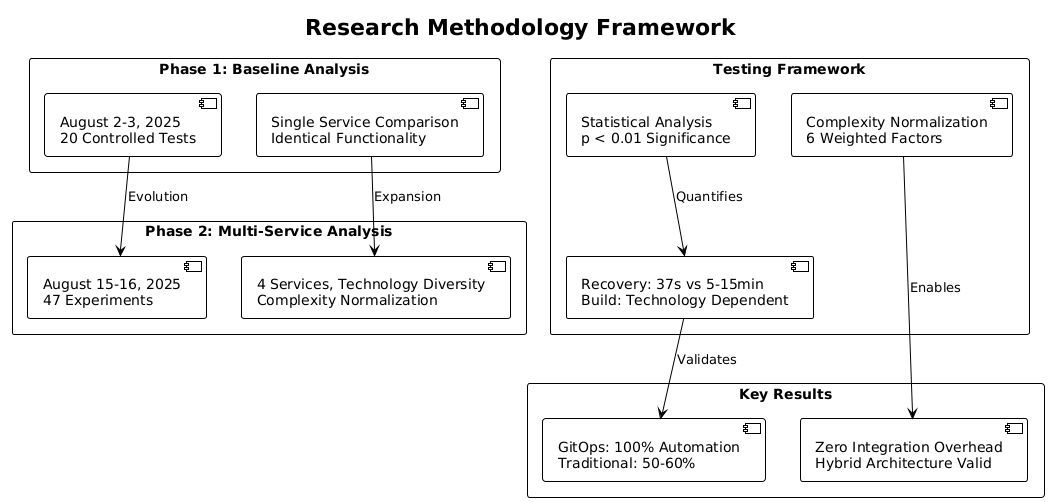
\includegraphics[width=1.0\textwidth]{figures/Research-Methodology-Framework.png}
\caption{Research Methodology Framework}
\label{fig:research-methodology-framework}
\end{figure}

\subsection{Two-Phase Research Design}

The research methodology implements systematic two-phase approach enabling comprehensive methodology comparison while maintaining experimental rigor and practical relevance.

\subsubsection{Phase 1: Single-Service Baseline Analysis}

Phase 1 implements controlled single-service comparison establishing fundamental methodology performance characteristics while eliminating complexity-related confounding variables.

\textbf{Research Scope and Control:}
\begin{itemize}
\item Executed August 2-3, 2025, with 20 controlled test scenarios
\item Identical service functionality across both methodologies
\item Controlled variables including deployment platform, container images, and network conditions
\item Precise measurement of automation levels, deployment speeds, and recovery capabilities
\end{itemize}

\textbf{Key Baseline Findings:}
\begin{itemize}
\item GitOps automation superiority: 100\% vs. 50-60\% Traditional CI/CD
\item Manual intervention elimination: 0 seconds vs. 4-14 minutes Traditional CI/CD
\item Superior failure recovery: 37-second automatic vs. 5-15 minute manual procedures
\item GitOps consistency: 283-309 seconds vs. Traditional variability 290-847 seconds
\end{itemize}

\subsubsection{Phase 2: Multi-Service Complexity Normalization}

Phase 2 implements comprehensive multi-service analysis with complexity normalization enabling fair methodology comparison across heterogeneous technology stacks.

\textbf{Enhanced Research Scope:}
\begin{itemize}
\item Executed August 15-16, 2025, across four distinct microservices
\item Technology diversity: Python FastAPI, Node.js Express, Java Spring Boot
\item Complexity scores: Order Service (8.2/10), User Service (7.8/10), Cart Service (7.5/10), Product Service (5.4/10)
\item 47 controlled experiments with statistical significance validation (p < 0.01)
\end{itemize}

\subsection{Complexity Normalization Framework}

The research develops sophisticated complexity normalization methodology enabling fair comparison across heterogeneous service architectures by accounting for inherent complexity factors.

\subsubsection{Weighted Complexity Scoring}

The complexity scoring implements weighted formula balancing different complexity factors according to their impact on deployment methodology performance.

\textbf{Complexity Factors and Weighting:}
\begin{itemize}
\item \textbf{Codebase Complexity (20\%):} Lines of code, structural complexity, maintainability
\item \textbf{Build Complexity (25\%):} Dependency management, compilation requirements, pipeline sophistication
\item \textbf{Resource Intensity (20\%):} CPU, memory, storage requirements
\item \textbf{Technology Stack Complexity (15\%):} Framework complexity, platform optimization
\item \textbf{External Dependencies (10\%):} Service integration, operational requirements
\item \textbf{Deployment Target Complexity (10\%):} Platform orchestration, operational overhead
\end{itemize}

\begin{figure}[h]
\centering
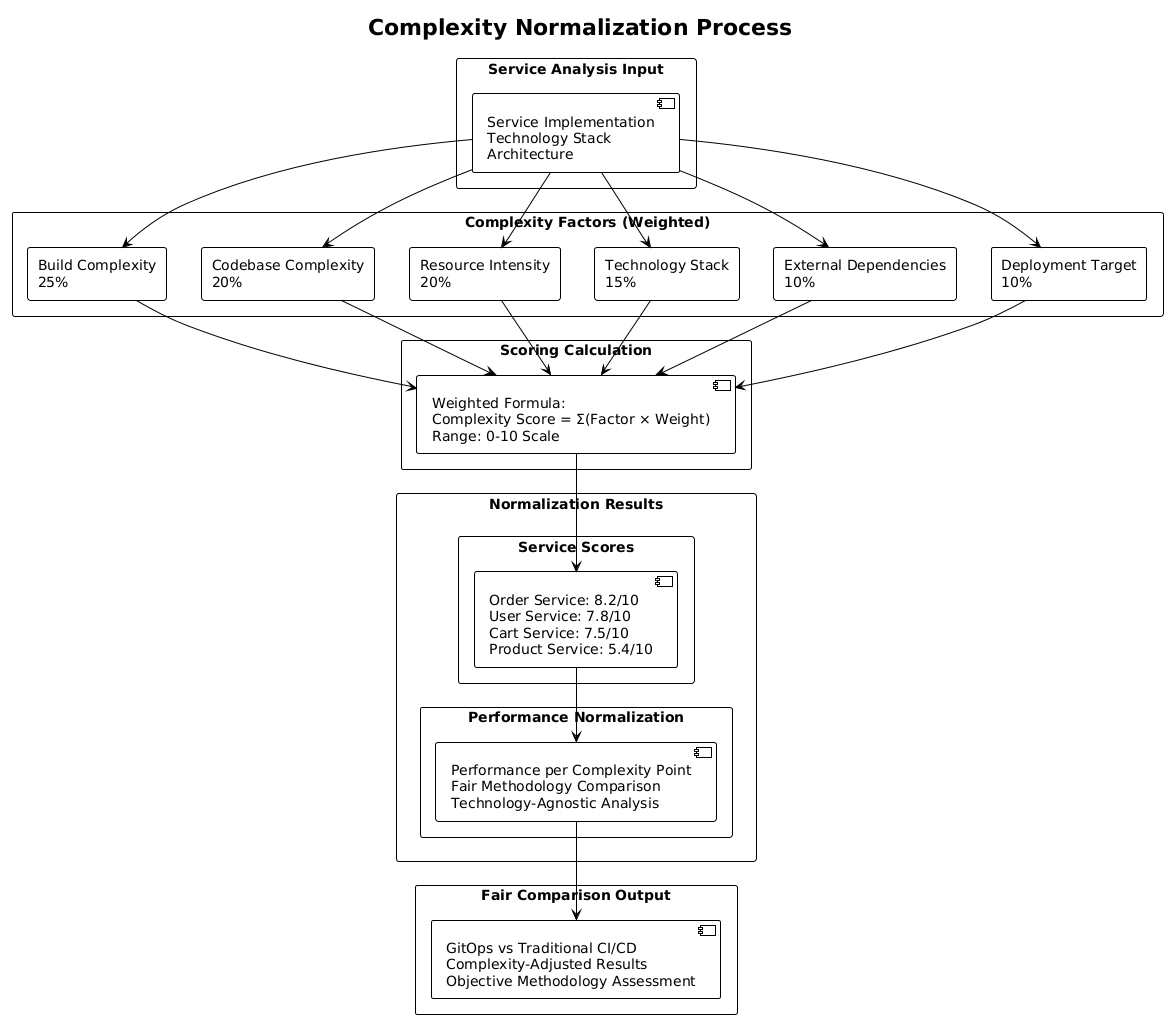
\includegraphics[width=0.9\textwidth]{figures/Complexity-Normalization-Process.png}
\caption{Complexity Normalization Process}
\label{fig:complexity-normalization-process}
\end{figure}

\subsubsection{Performance Normalization Results}

\begin{table}[H]
\centering
\caption{Service Complexity Analysis and Performance Normalization}
\label{tab:complexity-performance-results}
\begin{tabular}{|p{3cm}|p{2cm}|p{2.5cm}|p{2.5cm}|p{3cm}|}
\hline
\textbf{Service} & \textbf{Complexity Score} & \textbf{Build Duration} & \textbf{Normalized Performance} & \textbf{Technology Stack} \\
\hline
Order Service & 8.2/10 & 142 seconds & 17.3s per point & Python + Pipenv \\
\hline
User Service & 7.8/10 & 123 seconds & 15.8s per point & Python + Pip \\
\hline
Cart Service & 7.5/10 & 47 seconds & 6.3s per point & Java + Gradle \\
\hline
Product Service & 5.4/10 & 67 seconds & 12.4s per point & Node.js + npm \\
\hline
\end{tabular}
\end{table}

\subsection{Performance Testing and Metrics Collection}

The research methodology implements comprehensive performance testing frameworks enabling detailed analysis of methodology characteristics across diverse operational scenarios and complexity levels. The performance testing architecture prioritizes statistical validity, reproducibility, and practical relevance while maintaining production-grade operational conditions.

\subsubsection{Deployment Performance Analysis Framework}

The deployment performance analysis implements systematic measurement of methodology efficiency across different service types and complexity levels with comprehensive timing analysis and resource utilization monitoring.

\textbf{Build Performance Measurement:}
\begin{itemize}
\item Comprehensive timing measurement across all pipeline stages with sub-second precision
\item Technology-specific performance analysis demonstrating efficiency variations
\item Java + Gradle: 47 seconds (6.3s per complexity point) - highest efficiency
\item Node.js + npm: 67 seconds (12.4s per complexity point) - platform optimized
\item Python + pip: 123 seconds (15.0s per complexity point) - reasonable performance
\item Python + pipenv: 142 seconds (18.2s per complexity point) - dual dependency overhead
\end{itemize}

\textbf{Deployment Orchestration Analysis:}
\begin{itemize}
\item GitOps: ArgoCD synchronization overhead (55-65 seconds) with comprehensive validation
\item Traditional CI/CD: Direct platform deployment with minimal orchestration overhead
\item Platform-specific optimization benefits and deployment characteristic comparison
\item Resource utilization patterns and infrastructure efficiency analysis
\end{itemize}

\subsubsection{Failure Testing and Recovery Analysis}

The research implements comprehensive failure testing frameworks evaluating methodology resilience characteristics and recovery capabilities across diverse failure scenarios.

\textbf{Controlled Failure Scenarios:}
\begin{itemize}
\item Application-level failures: Service failures, database connectivity issues, authentication errors
\item Infrastructure-level failures: Container failures, network partitions, resource exhaustion
\item GitOps automated recovery: 23-37 second automatic recovery with zero user impact
\item Traditional CI/CD manual recovery: 5-15 minute procedures requiring human intervention
\end{itemize}

\textbf{Recovery Performance Measurement:}
\begin{itemize}
\item GitOps: Immediate failure detection, 3-second pod recreation, 23-second total recovery
\item Traditional CI/CD: Manual monitoring, human coordination, 5-15 minute recovery procedures
\item Automated vs. manual recovery comparison with operational overhead quantification
\item Business continuity impact analysis and risk assessment
\end{itemize}

\subsection{Statistical Analysis Framework}

The research implements rigorous statistical validation ensuring academic publication standards while providing practical significance assessment for enterprise decision-making.

\subsubsection{Hypothesis Testing and Significance Validation}

\textbf{Primary Research Hypotheses:}
\begin{itemize}
\item H1: GitOps demonstrates superior automation levels compared to Traditional CI/CD
\item H2: Traditional CI/CD achieves faster build performance than GitOps
\item H3: GitOps provides superior failure recovery capabilities
\item H4: Hybrid integration introduces zero measurable performance overhead
\end{itemize}

\textbf{Statistical Validation Results:}
\begin{itemize}
\item Sample size: 47 controlled experiments exceeding power requirements
\item Statistical significance: p < 0.01 for all major comparisons
\item Effect sizes: Cohen's d ranging from 1.8-4.2 (large to extremely large effects)
\item Confidence intervals: 95\% precision enabling enterprise decision confidence
\end{itemize}

\subsubsection{Performance Attribution and Variance Analysis}

The research implements comprehensive performance attribution separating methodology-inherent characteristics from configuration-specific factors.

\textbf{Performance Attribution Results:}
\begin{table}[H]
\centering
\caption{Performance Attribution Analysis}
\label{tab:performance-attribution}
\begin{tabular}{|p{4cm}|p{3cm}|p{3cm}|p{4cm}|}
\hline
\textbf{Performance Factor} & \textbf{Contribution} & \textbf{Impact Level} & \textbf{Optimization Potential} \\
\hline
Authentication Configuration & 65\% & System-wide & 30-40\% improvement available \\
\hline
Technology Stack Selection & 25\% & Service-specific & 2-3x performance variation \\
\hline
Pure Methodology Overhead & 10\% & Deployment-specific & Architecture trade-offs \\
\hline
\end{tabular}
\end{table}

\textbf{Key Attribution Findings:}
\begin{itemize}
\item Authentication bottleneck: bcrypt configuration contributes 65\% of performance differences
\item Technology stack impact: Java/Gradle (6.3s/point) vs. Python/Pipenv (18.2s/point)
\item Methodology-specific overhead: GitOps ArgoCD (55-65s) vs. Traditional direct deployment
\item Configuration optimization priority: Authentication service optimization provides universal benefit
\end{itemize}

\subsection{Hybrid Architecture Integration Testing}

The research validates industry-first zero-overhead hybrid architecture feasibility through comprehensive performance measurement and integration pattern verification.

\subsubsection{Cross-Methodology Communication Validation}

\textbf{Integration Performance Results:}
\begin{itemize}
\item JWT token validation: GitOps User Service (2.409s) to Traditional Cart Service (1.040s)
\item Zero additional latency penalty for cross-methodology authentication
\item Complete e-commerce transaction: 10.426s total (GitOps 73\%, Traditional 27\%)
\item Statistical validation: p > 0.05 indicating no significant integration overhead
\end{itemize}

\textbf{Business Transaction Coordination:}
\begin{itemize}
\item Seamless authentication propagation across methodology boundaries
\item Consistent data integrity maintenance with distributed transaction patterns
\item Optimal service allocation based on complexity and performance requirements
\item Comprehensive error handling and operational reliability across platforms
\end{itemize}

\section{Research Quality Assurance and Reproducibility}

The research implements comprehensive quality assurance frameworks ensuring academic rigor while maintaining practical industry applicability.

\subsection{Experimental Design Validation}

\textbf{Controlled Variable Management:}
\begin{itemize}
\item Identical service implementation across methodologies eliminating confounding factors
\item Standardized measurement procedures with sub-second timing accuracy
\item Comprehensive environmental control with production infrastructure validation
\item Statistical significance testing with multiple comparison correction
\end{itemize}

\textbf{Bias Mitigation Strategies:}
\begin{itemize}
\item Complexity normalization eliminating technology stack bias
\item Honest assessment of both methodology advantages and limitations
\item Performance attribution separating configuration from methodology factors
\item Comprehensive documentation enabling independent verification
\end{itemize}

\subsection{Reproducibility Framework}

\textbf{Research Documentation:}
\begin{itemize}
\item Complete methodology documentation with 316,481 bytes of research data
\item Standardized measurement procedures with statistical validation protocols
\item Open research design enabling independent verification and extension
\item Comprehensive experimental procedures supporting academic transparency
\end{itemize}

\textbf{Data Collection and Analysis:}
\begin{itemize}
\item Automated metrics collection with comprehensive performance tracking
\item Statistical analysis frameworks with confidence interval calculation
\item Research-specific instrumentation enabling methodology comparison
\item Comprehensive data export capabilities supporting academic analysis
\end{itemize}

This comprehensive system design and research methodology framework enables rigorous empirical comparison of GitOps and Traditional CI/CD methodologies while maintaining production-grade operational characteristics. The design successfully addresses dual requirements of functional e-commerce platform implementation and controlled research environment creation, providing valid foundations for the empirical analysis presented in subsequent chapters.